Cryptographic signatures are used to prove the validitiy of an encrypted message.
Suppose Alice wants to send an encrypted message to Bob, but Eve wants to intercept
or obfuscate such a message.  Alice could use an ecryption algorithm such as AES,
then send the message to Bob.  However, it is entirely possible that Eve intercepts
the encrypted message while it is en route to Bob.  While it would be computationally
difficult for Eve to crack the encrypted message, Eve could alter the encrypted message
such that Bob would not be able to unencrypt the message. Furthermore, Eve could get lucky
and somehow obtain the AES key used by Alice and Bob. In both of these cases, Alice and Bob
would benefit form using some form of digitial signature method.  Digital signatures
are used to prove the authenticity and validity of a message.  In general, this is done by
signing the hash of a message, and sending this signed hash together with and encrypted message.
The hash of the message ensures that the message has not been
tampred with.  The fact that the hash is signed ensures that the message is in fact coming
from the person who signed the message, and no one else.

DSA, the Digital Signature Algorithm, is a common method of signing messages.
The structure of DSA has been augmented to take advantage of the
computationally difficult aspect of pointwise addition and scalar multiplication
on elliptic curves.  In this section, we will explain the multiplication
and addition for elliptic curves, why this would be difficult to reverse,
and finally describe the actual ECDSA algorithm.

\subsection{Elliptic Curve Theory}

Elliptic curves are complicated geometric and algebraic objects,
whose full explanation lies outside the scope of this paper.
The purpose of this section is to provide a vague understanding
of why elliptic curve cryptography might be secure, so that the reader
can have a top level understanding of how the iMessage protocol
works, and is secure.\\

An elliptic curve is an equation in the form $y^2 = x^3 + ax^2 + bx + c$.

When working with elliptic curves, it is often most useful to describe the curve as a set
$$\{(x,y) \vert x,y \in K, y^2 = x^3 + ax^2 + bx + c\} \cup \{ \infty \}$$, where $K$ is a set such as
$\mathbb{Q}, \mathbb{R}, \mathbb{Z} \mod p$, where $p$ is prime.

We include a point at
$\infty$, which serves as the identity under point addition.
Conceptually, we think of as lines through $\infty$
as vertical lines.

The elliptic curves with cryptographic applications are ones where $K$ is the integers
mod a prime $p$, denoted $\mathbb{F}_p$.

\begin{example}
    Consider the elliptic curve $E = y^2 = x^3+2x-1 \mod 5$.

    Using the set notation, we can describe this curve as
    $E = \{(0 ,2 ),(0,3),(2,1),(2 ,4 ),(4,1),(4,4), \infty\}$.
\end{example}




\subsubsection{Adding Points of an Elliptic Curve}
Suppose we want to add points $P_1$ and $P_2$.

The following algorithm serves as addition on elliptic curve points.
\begin{algorithm}
    \begin{algorithmic}
        \Procedure{(+)}{$P_1,P_2$}
        \If{$P_1 == P_2$}
        \State $L \gets$ the line tangent to $E$ intersecting $P_1$
        \Else
        \State $L \gets$ the line through both $P_1$ and $P_2$
        \EndIf
        \State $R \gets$ the intersection of $L$ and $E$, $R \neq P_1, P_2$
        \State Suppose $R = (r_x, r_y)$
        \State \textbf{return} $(r_x, -r_y)$
        \EndProcedure
    \end{algorithmic}
    \caption{Adding $P_1$ and $P_2$ on an elliptic curve $E$}
    \label{euclid}
\end{algorithm}

The existence of such a point $R$ is given by the properties of elliptic curves,
so this operation is well defined.

\begin{example}

    We will show how to compute $P + Q$ on the given elliptic curve in Figure \ref{adding}.

    We start by drawing the line through both $P$ and $Q$.

    The intersection of this line is point $R$.  We then reflect $R$ across the
    $x$-axis, resulting in $P + Q$.

    \begin{figure}[h!]
        \caption{Adding points $P$ and $Q$ on an elliptic curve \cite{kakaroto}}\label{adding}
        \centering
        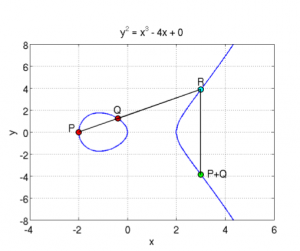
\includegraphics[width=0.5\textwidth]{elliptic_curve_addition.png}
    \end{figure}

\end{example}





\begin{example}
As mentioned previously, there is an $\infty$ point that serves as the additive identity.

Consider $(x,y) + \infty$.

The line through $(x,y)$ and $\infty$ will be completely vertical.

So the point of intersection (labeled $R$ in the algorithm) will be $(x,-y)$.

Then, following the algorithm, we get that $(x,y) + \infty = (x,y)$.

Thus $\infty$ is the additive identity for an elliptic curve.
\end{example}




\subsection{The Discrete Logarithm Problem}

\subsubsection{The classic Discrete Log Problem}
A variant of the discrete logarithm problem is the foundation of elliptic
curve cryptography.  The classic discrete logarithm problem is as follows:\\

Consider an arbitrary group $(G, *)$ and suppose $b,g \in G$.

The discrete logarithm problem is to find an integer $k$
such that $b^k = g$.

Finding such a $k$ is computationally difficult; yet
with $k$ known, it is very simple to compute $b^k$.

Since exponentiation is the easy part of an invertible function, with
the logarithm being difficult to compute, this problem has cryptographic
applications.


\subsubsection{The Discrete Logarithm Problem for Elliptic Curves}

Consider an elliptic curve $E$ with points $A,B$.

The elliptic curve discrete Logarithm problem to find $k$
such that $B = kA$.

Analogous to the classic discrete logarithm problem, finding such a $k$
is computationally difficult, but computing $B$ is relatively simple.

The discrete logarithm problem for elliptic curves is the foundation of
elliptic curve cryptography.

\subsection{DSA with Elliptic Curves}

Suppose Alice want to send a message to Bob, that has been signed with ECDSA.
First, the two of them will need to agree on an elliptic curve equation, call it $C$.
Additionally, they must agree on an element, call it $G$, that generates $C$ under
point-wise addition.  Finally, the order of the element $G$ (the number of times we must add
$G$ to itself before we generate the entire group) must be known. In order for ECDSA to be
secure, we want $n$ to be large.


\subsubsection{Signing a Message}

Alice starts with a public key $d_A \gets$ a random integer in $[1, n-1]$
and a public point on $C$, called $Q_A$.

\begin{algorithm}
    \begin{algorithmic}[1]
        \Procedure{ECDSA}{$M$}
        \State $e \gets \text{HASH}(m)$
        \State Suppose $n$, when represented as an unsigned binary number, has $L_n$ bits.
        Then $z \gets$ the $L_n$ leftmost bits of $e$.
        \State $k \gets$ a random integer in $[1, n-1]$.
        \State $(x,y) \gets k \times G$
        \State $r \gets x \mod n$
        \If {$r == 0$}
        \State Go to 4
        \EndIf
        \State $s \gets k^{-1}(z + rd_A) \mod n$
        \If {$s == 0$}
        \State Go to 4
        \EndIf
        \State \textbf{return} $(r, s)$
        \EndProcedure
    \end{algorithmic}
    \caption{Signing a message with ECDSA}
\end{algorithm}


\subsubsection{Verifying a Message}

Alice starts with a public key $d_A \gets$ a random integer in $[1, n-1]$
and a public point on $C$, called $Q_A$.

\begin{algorithm}
    \begin{algorithmic}[1]
        \Procedure{ECDSA}{$M$}
        \State $e \gets \text{HASH}(m)$
        \State Suppose $n$, when represented as an unsigned binary number, has $L_n$ bits.
        Then $z \gets$ the $L_n$ leftmost bits of $e$.
        \State $k \gets$ a random integer in $[1, n-1]$.
        \State $(x,y) \gets k \times G$
        \State $r \gets x \mod n$
        \If {$r == 0$}
        \State Go to 4
        \EndIf
        \State $s \gets k^{-1}(z + rd_A) \mod n$
        \If {$s == 0$}
        \State Go to 4
        \EndIf
        \State \textbf{return} $(r, s)$
        \EndProcedure
    \end{algorithmic}
    \caption{Signing a message with ECDSA}
\end{algorithm}


